\clearpage
\section{Cronómetro} \label{sec:crono}

Con el \emph{Hello World!!!} hemos visto como crear nuestro proyecto y una de las características más potentes de Angular, el \emph{Data Binding}. Ahora vamos a dar un pasito más y vamos crear una aplicación que sirva como cronómetro. Para ello, además de usar el \emph{Data Binding}, que por otro lado va a estar presente en la mayoría de desarrollos, veremos como modificar datos desde la lógica del componente y que estos cambias se vean reflejados en la vista. Además introduciremos algunas directivas de Angular, como es \textbf{*ngFor}, que utilizaremos para recorrer listas que formen parte del componente desde la propia plantilla

El primer paso, como no podría ser de otra manera, será crear un nuevo proyecto en blanco dentro de nuestro directorio de trabajo, de la misma forma que vimos en el capítulo anterior sobre el \nameref{sec:hello}:

\begin{lstlisting}[language=bash]
  # ionic start Chronometer blank --v2
\end{lstlisting}

En primer lugar vamos a hacer un cronómetro que tenga como unidad de medida mínima el segundo. También añadiremos dos botones, uno que actuará como Start/Pause para iniciar y detener el cronómetro, y otro que actuará como Stop, y que pondrá a cero de nuevo el cronómetro.

En la página web oficial de Ionic podemos encontrar una sección dedicada a los componentes\footnote{\url{https://ionicframework.com/docs/v2/components}} que nos ofrece el framework. Aquí podremos encontrar el componente que se utiliza para poder crear un botón, y las opciones que permite, como por ejemplo las dimensiones. También podremos encontrar una sección, llamada \emph{Ionicons}\footnote{\url{https://ionicframework.com/docs/v2/ionicons/}}, en la que encontraremos iconos que ofrece el propio framework. Lo interesante de estos iconos es que se adaptan según la plataforma es la que se ejecuta la aplicación, haciendo que el \emph{Look and Feel} de esta sea coherente con la plataforma en cuestión.

\begin{figure}[H]
\centering
  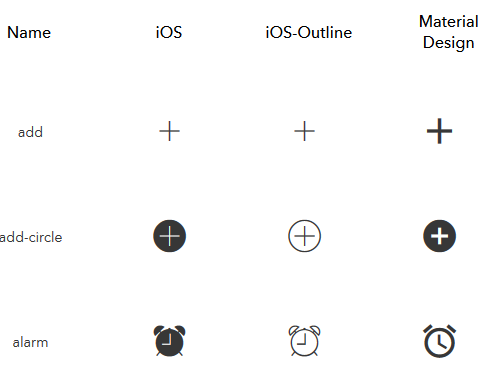
\includegraphics{Figures/ch2/Chronometer/ionicons}
  \caption{Una pequena parte de los iconos que ofrece Ionicons. Podemos ver la diferencia que existen entre ambas plataformas.}
\end{figure}

Empezaremos editando el fichero \emph{home.html} y creando un cronómetro con los elementos que queramos que lo compongan. De momento usaremos valores fijos, sin añadir ningún tipo de lógica, pudiendo así ver como queda el diseño escogido. Aquí cada cual puede utilizar el diseño que quiera, en mi caso, he optado por uno sencillo:

\begin{lstlisting}[style=htmlcssjs,frame=tlrb,xleftmargin={0.2cm}]
  <ion-content padding>
    <p style="text-align: center; font-size: -webkit-xxx-large;" >
      00:00:00
    </p>

    <ion-row>
      <ion-col>
        <button ion-button  color="secondary" full large >
          <ion-icon name="play" ></ion-icon>
          Start
        </button>
      </ion-col>
    </ion-row>

    <ion-row>
      <ion-col>
        <button ion-button color="danger" full large >
          <ion-icon name="square" ></ion-icon>
          Stop
        </button>
      </ion-col>
    </ion-row>
  </ion-content>
\end{lstlisting}

Con este diseño, nuestra página se vera tal que así:

\begin{figure}[H]
\centering
  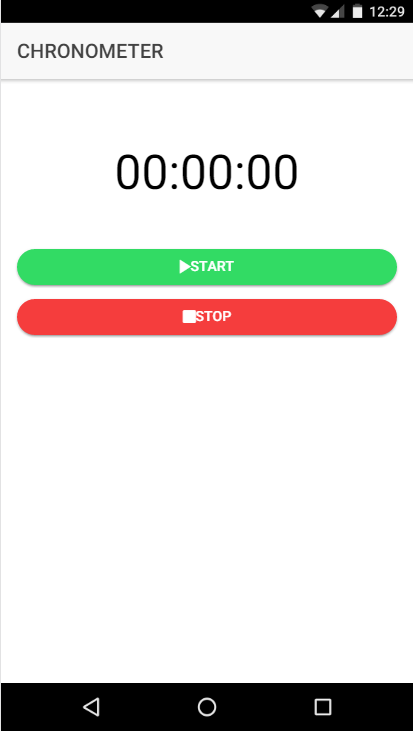
\includegraphics[width=0.4\textwidth]{Figures/ch2/Chronometer/1}
  \caption{Esto sí que es un cronómetro sencillo.}
\end{figure}

\notebox{El navegador Chrome nos da la opción de simular la vista de un dispositivo móvil y poder así comprobar como se ve nuestra aplicación limitada a diferentes tamaños de pantalla. Para ello, tendremos que abrir la herramienta para desarrolladores pulsando F12, y activamos \emph{Device Toolbar} con el botón 
\includegraphics{Figures/ch2/Chronometer/toggle_device_toolbar} o pulsando Ctrl+Shift+M. Esto nos abrirá una barra superior en la que podremos elegir entre diferentes modelos de dispositivos o definir el tamaño de la pantalla en píxeles manualmente.
Aunque por lo general suele ser un comportamiento cercano a la realidad, en ocasiones el resultado visto aquí y el que después vemos en la realidad puede variar en lo referente a dimensiones y posiciones de algunos elementos.}

Siguiente paso, añadir lógica a nuestra aplicación, para ello vamos a editar el fichero \emph{home.component.ts}. En este fichero \emph{TypeScript} encontramos la clase \emph{HomePage}, la cual esta precedida por el decorador \emph{@Component} de Angular. Esto quiere decir que esta clase se trata de un componente de Angular. Es este decorador se definirán los metadatos del componente, en este caso, se han definido dos de ellos: el \emph{template} y el \emph{selector}, los cuales indican el código o fichero \gls{HTML} que define el aspecto visual del componente en el caso del \emph{template} y el nombre del tag \gls{HTML} que representa este controlador en el caso del \emph{selector}. Gracias al \emph{Data Binding}, las propiedades y métodos que definamos dentro de este controlador, serán accesibles desde el código \gls{HTML} si es necesario. En primer lugar, vamos a pensar que variables precisamos para la implementación del cronómetro:

\begin{itemize}
  \item Un \emph{flag} que nos indique si el cronómetro está o no en marcha.
  \item Un contador para que almacene los segundos desde la puesta en marcha.
  \item Para que el botón Start/Pause cambie según el estado, necesitaremos hacerlo usando dos variables:
  \begin{itemize}
    \item Una cadena de texto que almacene la el texto que aparece en el botón: \emph{Start} o \emph{Pause}
    \item Una cadena que indique que icono usar en el botón.
  \end{itemize}
\end{itemize}

Todas estás variables serán inicializadas en el constructor. Para cumplir con esto requisitos utilizamos el siguiente código:

\begin{lstlisting}[style=htmlcssjs,frame=tlrb,xleftmargin={0.2cm}]
  _is_running:boolean;
  seconds:number;
  start_pause_label: string;
  start_pause_icon: string;

  constructor() {
    this.is_running = false;
    this.seconds = 0;
  };
\end{lstlisting}

\tipbox{Es una práctica recomendable que los nombres de las propiedades, de las funciones, de las clases, \ldots sean autodescriptivos, ya estemos trabajando con TypeScript como con cualquier otro lenguaje.}

No hemos inicializado ni \emph{start\_pause\_label} ni \emph{start\_pause\_icon} por la siguiente razón, estas variables están ligadas al estado en que se encuentra el cronómetro, es decir a \emph{\_is\_running}. Para asegurarnos que estos valores cambian al cambiar \emph{\_is\_running}, vamos a personalizar el \emph{getter} y el \emph{setter}\footnote{\url{https://www.typescriptlang.org/docs/handbook/classes.html#accessors}} de esta propiedad, esta es la razón por la que se ha prefijado el nombre de la propiedad con una barra baja (\_) evitando así el conflicto que se produciría con los nombres. Los métodos quedarían de la siguiente manera:

\begin{lstlisting}[style=htmlcssjs,frame=tlrb,xleftmargin={0.2cm}]
  public get is_running() {
    return this._is_running;
  };

  public set is_running(new_state) {
    this._is_running = new_state;
    this.start_pause_label = this.is_running ? "Pause" : "Start";
    this.start_pause_icon = this.is_running ? "pause" : "play";
  };
\end{lstlisting}

Cada vez que se haga una consulta a la propiedad \emph{is\_running}, se ejecutará la primera función, y cuando se asigne un valor (como ocurre en el constructor al ejecutar \emph{this.is\_running = false;}), se ejecutará la segunda función, la cual asigna el nuevo valor a \emph{is\_running}, y según sea este, a \emph{start\_pause\_label} y \emph{start\_pause\_icon}.

Llega el momento de implementar los métodos, para lo cual vamos a realizar un ejercicio anterior a la codificación similar al que hicimos con las propiedades. Los métodos que considero necesarios son para conseguir hacer funcionar nuestro cronómetro son:

\begin{itemize}
  \item Un método que sirva para cambiar el estado del cronómetro y que funcione si fuera un interruptor.
  \item Otro que sirva para detener el cronómetro y ponerlo a 0 el contador.
  \item Un último método que aumente en 1 los segundos si cronómetro está en marcha.
\end{itemize}

Al implementar estos métodos, nos quedará el componente de la siguiente manera:

\begin{lstlisting}[style=htmlcssjs,frame=tlrb,xleftmargin={0.2cm}]
  export class HomePage {
    private _is_running:boolean;
    seconds:number;
    start_pause_label: string;
    start_pause_icon: string;

    constructor() {
      this.is_running = false;
      this.seconds =0;

      setInterval(() => {
        this.tick();
      }, 1000);
    };

    public get is_running() {
      return this._is_running;
    };

    public set is_running(new_state) {
      this._is_running = new_state;
      this.start_pause_label = this.is_running ? "Pause" : "Start";
      this.start_pause_icon = this.is_running ? "pause" : "play";
    };

    tick(): void {
      if (this.is_running) {
        this.seconds++;
      }
    };

    toggle(): void {
      this.is_running = !this.is_running;
    };

    stop(): void {
      this.is_running = false;
      this.seconds = 0;
    };
  }
\end{lstlisting}

Para que la función \emph{tick()} tenga sentido, es necesario que se ejecute cada segundo. Vamos a usar la función \emph{setInternal()}. Esta función es nativa de JavaScript y por ello podemos hacer uso de ella desde TypeScript. La invocamos en el constructor indicando el método al que tiene que llamar y la espera entre una llamada y otra (el tiempo que se le pasa debe estar expresado en milisegundos):

\begin{lstlisting}[style=htmlcssjs,frame=tlrb,xleftmargin={0.2cm}]
  constructor() {
    // RESTO DE FUNCIÓN
    setInterval(() => {
      this.tick();
    }, 1000);
  };
\end{lstlisting}

Otra opción sería llamar a la función \emph{setInternal()} en el \emph{setter} de \emph{is\_running} y asignar el id devuelto a una variable del controlador, y así poder desactivarlo con la función \emph{clearInterval()}, la cual acepta como parámetro el ID anterior. Algo como:


\begin{lstlisting}[style=htmlcssjs,frame=tlrb,xleftmargin={0.2cm}]
  public set is_running(new_state) {
    this._is_running = new_state;
    if (this.is_running) {
      this.start_pause_label = "Pause"
      this.start_pause_icon = "pause"
      this.interval_id = setInterval(() => {
        this.tick();
      }, 1000);
    } else {
      this.start_pause_label = "Start"
      this.start_pause_icon = "play"
      clearInterval(this.interval_id);
    }
  };
\end{lstlisting}

La ventaja de esta opción es que se evita la llamada a la función \emph{tick()} cuando el cronómetro está detenido.

Con la lógica ya implementada, vamos a conectar las propiedades del componente con los elementos de la template, y para ello nos ayudaremos del famoso \emph{Data Binding}. Como nuestra template esta asignada al componente definido por la clase \textbf{HomePage}, podremos hacer uso de sus propiedades y métodos. Para hacer funcionar el cronómetro, necesitaremos:

\begin{enumerate}
  \item Por un lado modificar los valores mostrados en el \gls{HTML} para que coincidan con los definidos en el componente. Esto se hace poniendo el nombre de la variable o del método entre llaves dobles ( \{\{ NOMBRE \}\} ) en el \gls{HTML} allí donde queramos que el valor aparezca.
  \item Vincular el evento de \emph{click} sobre los botones a alguno de los métodos. Esto se consigue gracias a la directiva \textbf{(clic)} que se pone como atributo \gls{HTML} en el botón.
\end{enumerate}

El código se vería de la siguiente manera:

\begin{lstlisting}[style=htmlcssjs,frame=tlrb,xleftmargin={0.2cm}]
  <p style="text-align: center; font-size: -webkit-xxx-large;" >
    {{ seconds }}
  </p>

  <ion-row>
    <ion-col>
      <button ion-button  color="secondary" full large (click)="toggle()" >
        <ion-icon name="{{ start_pause_icon }}" ></ion-icon>
        {{ start_pause_label }}
      </button>
    </ion-col>
  </ion-row>

  <ion-row>
    <ion-col>
      <button ion-button color="danger" (click)="stop()" style="width: 100%;" >
        <ion-icon name="square" ></ion-icon>
        Stop
      </button>
    </ion-col>
  </ion-row>
\end{lstlisting}

Vemos que hemos cambiado el display donde se visualizan los segundos, el icono y el texto del boton ``Start''/``Pause'', se han añadido las directivas \emph{(clic)} para que hagan llamadas a las funciones que implementamos en nuestra clase \emph{HomePage} \ldots pero vemos que la forma de visualizar el tiempo transcurrido no es la que teníamos en mente, si no que vemos el número que utilizamos para contar los segundos desde el inicio, lo cuál no es intuitivo a la hora de leerlo.

Necesitamos por tanto, darle un formato más legible. Para esto vamos a usar otra herramienta que nos ofrece Angular, las llamadas \emph{Pipes o tuberias}.

El concepto de \emph{Pipe} es similar al que se utiliza por ejemplo en \emph{bash} o \emph{sh}, y nos permite transformar un dato, el cual se le pasa como entrada a la tubería, y obtenemos el mismo dato ya transformado. Para nuestra aplicación necesitamos que nuestros segundos, que no es más que un número que representa la cantidad de segundos desde el inicio a nivel lógico, se convierta en una cadena de texto con un formato más amigable para el usuario, \emph{0h 00m 00s}. Angular dispone de algunos \emph{Pipes} ya definidos\footnote{\url{https://angular.io/docs/ts/latest/api/#!?query=pipe}}, pero en nuestro caso, definiremos uno propio.

Empezaremos creando un nuevo fichero \emph{.ts} al que llamaremos \emph{home.pipes.ts}. Con esto conseguimos que el código quede MAS ORDENADO. Dentro de este fichero crearemos nuestra clase, la cual deberá implementar la interfaz \textbf{PipeTransform} y ser decorada con \emph{@Pipe}. Al implementar la interfaz \textbf{PipeTransform} tendremos que definir el método \textbf{transform()}. Este será el método que se ejecute cuando nuestra tubería sea usada, pasando la entrada de esta como parámetro. El decorador \emph{@Pipe} acepta el argumento \textbf{name}, el cuál nos permite asignar un identificador a nuestra tubería.

\begin{lstlisting}[style=htmlcssjs,frame=tlrb,xleftmargin={0.2cm}]
  @Pipe({name: 'time_format'})
  export class MyTimePipe implements PipeTransform {
    transform(seconds: number): string {
      var s_num = seconds % 60;
      var m_num = Math.floor((seconds % 3600) / 60);
      var h_num = Math.floor(seconds / 3600);

      var s = ('0' + s_num).slice(-2);
      var m = ('0' + m_num).slice(-2);
      var h = '' + h_num;

      return '\${h}h \${m}m \${s}s';
    }
  }
\end{lstlisting}

Ya solo nos queda utilizar esta tubería en nuestro template. Cambiamos la llamada a la variable \emph{seconds} para que pase por nuestra tubería:

\begin{lstlisting}[style=htmlcssjs,frame=tlrb,xleftmargin={0.2cm}]
  <p style="text-align: center; font-size: -webkit-xxx-large;" >
    {{ seconds | time_format }}
  </p>
\end{lstlisting}

Al utilizar esta tubería, conseguimos que el contador de segundos siga siendo un número, lo que facilita su uso en otras partes del código. También tenemos disponible un método sencillo y reusable para convertir segundos a un formato entendible para el usuario y que volveremos a usar en el siguiente apartado.

\subsection{Cronómetro con contador de vuelta}

Vamos a añadir una función extra a nuestro cronómetro, un contador de vueltas. Este contador nos permitirá guardar el registro en un momento dado sin detener el cronómetro. Estos registros que se vayan guardando aparecerán en una lista debajo de la botonera, la cuál también modificaremos para añadir dos nuevos botones.

\begin{figure}[H]
\centering
  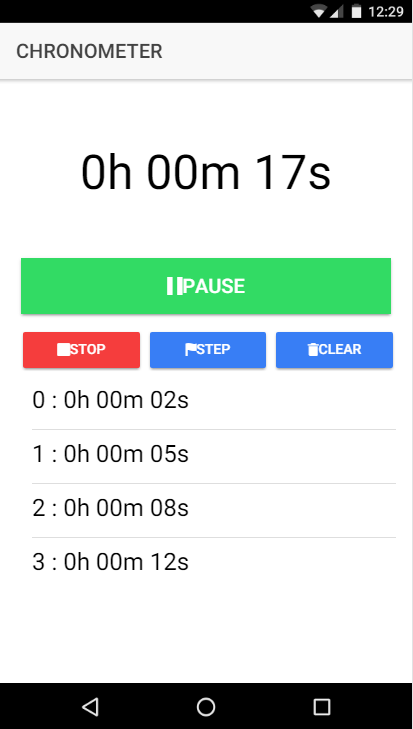
\includegraphics[width=0.4\textwidth]{Figures/ch2/Chronometer/chronometer_v2}
  \caption{En esta nueva versión hemos añadido dos nuevos botones además de una lista con los tiempos guardados.}
\end{figure}

Veamos a continuación las modificaciones hechas a nuestro \gls{HTML} para introducir los nuevos botones y la lista.

\begin{lstlisting}[style=htmlcssjs,frame=tlrb,xleftmargin={0.2cm}]
  <ion-content padding>
  <p style="text-align: center; font-size: -webkit-xxx-large;" >
    {{ seconds | time_format }}
  </p>

  <ion-row>
    <ion-col>
      <button ion-button  color="secondary" full large (click)="toggle()" >
        <ion-icon name="{{ start_pause_icon }}" ></ion-icon>
        {{ start_pause_label }}
      </button>
    </ion-col>
  </ion-row>

  <ion-row>
    <ion-col>
      <button ion-button color="danger" (click)="stop()" style="width: 100%;" >
        <ion-icon name="square" ></ion-icon>
        Stop
      </button>
    </ion-col>
    <ion-col>
      <button ion-button (click)="step()" style="width: 100%;" >
        <ion-icon name="flag" ></ion-icon>
        Step
      </button>
    </ion-col>
    <ion-col>
      <button ion-button (click)="clear()" style="width: 100%;" >
        <ion-icon name="trash" ></ion-icon>
        Clear
      </button>
    </ion-col>
  </ion-row>
  <ion-list>
    <ion-item  *ngFor="let step of step_list; let i=index" >
      <h1>{{ i }} : {{ step  | time_format }}</h1>
    </ion-item>
  </ion-list>
  </ion-content>
\end{lstlisting}

Los botones no tienen más misterio que los que se explicaron antes, cambiando la función a la que llaman, las cuales implementaremos más adelante.

Sí que nos encontramos dos componente nuevos de Ionic, \textbf{ion-list} y \textbf{ion-item}. Como bien se puede intuir por sus nombre, estos componentes sirven para crear listas y elementos dentro de ellas. Dentro del componente ion-item también vemos el atributo \textbf{*ngFor}. Este atributo se trata de una directiva de Angular que nos permite recorrer una lista, que definiremos en el componente, y por cada iteración renderizará el elemento que contiene la directiva, en este caso, el ion-item. En cada iteración sobre la lista, el valor recuperado se almacena en una variable (let step of step\_list) a la que se puede acceder del mismo modo que si se tratara de una propiedad del componente, pudiendo tratarla con nuestra tubería personalizada de igual manera que hacíamos con los segundos. Como opción, podemos recuperar el índice, que representa la posición que ocupa el elemento en la lista, y asignarlo a una variable (let i=index) que como no, también podemos usar como la anterior.

En lo que respecta a la lógica, necesitaremos implementar las dos funciones a las que se llamarán desde los nuevos botones, y una lista que almacene los registros que vayamos guardando. Desde una de las funciones haremos que se añada a la lista el tiempo actual, desde la otra limpiaremos la lista. Como ocurre con el resto de propiedades, cada vez que modifiquemos la lista, se actualizará la vista de la misma manera que pasaba con los segundos, sin importar que la variable se encuentre dentro de la directiva *ngFor.

\begin{lstlisting}[style=htmlcssjs,frame=tlrb,xleftmargin={0.2cm}]
  export class HomePage {
    // RESTO DE VARIABLES
    step_list: number[];

    // RESTO DE FUNCIONES
    step(): void {
      if (this.is_running) {
        this.step_list.push(this.seconds);
      }
    }

    clear(): void {
      this.step_list = [];
    }
  }
\end{lstlisting}

Estas nuevas funciones serán ejecutadas cada vez que pulsemos sobre los correspondientes botones ya que como vimos antes, han sido asignados utilizando la directiva \textbf{(click)}.
